\documentclass{article}
\usepackage{graphicx}
\usepackage{hyperref}
\usepackage{amsmath}
\usepackage{cite}

\title{Guitar Pedal Effects}
\author{}
\date{}

\begin{document}

\maketitle

\section{Introduction}
This document describes the mathematical basis of various guitar pedal effects and provides figures on how to select and configure these effects.

\section{Common Guitar Effects}
\subsection{Tremolo}
The technical name for the tremolo effect is amplitude modulation. This effect is achieved by multiplying a waveform with a triangle wave.

\begin{equation}
y(t) = x(t) \cdot (1 + \sin(2 \pi f t))
\end{equation}

\subsection{Distortion \& Overdrive}
Distortion is a general term for any modification to an audio signal that provides significant alteration. Most distortion effects use clipping and overtones on a signal to alter the input wave. Overdrive works by increasing the gain at specific outputs past the threshold.

\begin{equation}
y(t) = \begin{cases} 
      x(t) & \text{if } |x(t)| < T \\
      T \cdot \text{sgn}(x(t)) & \text{if } |x(t)| \geq T 
   \end{cases}
\end{equation}

\subsection{FUZZ}
This effect takes whatever waveform is input and forces it into a square waveform.

\begin{equation}
y(t) = \text{sgn}(x(t))
\end{equation}

\subsection{DELAY}
This is where the waveform is played and then repeated with a lower amplitude.

\begin{equation}
y(t) = x(t) + \alpha x(t - \tau)
\end{equation}

\begin{figure}[h]
    \centering
    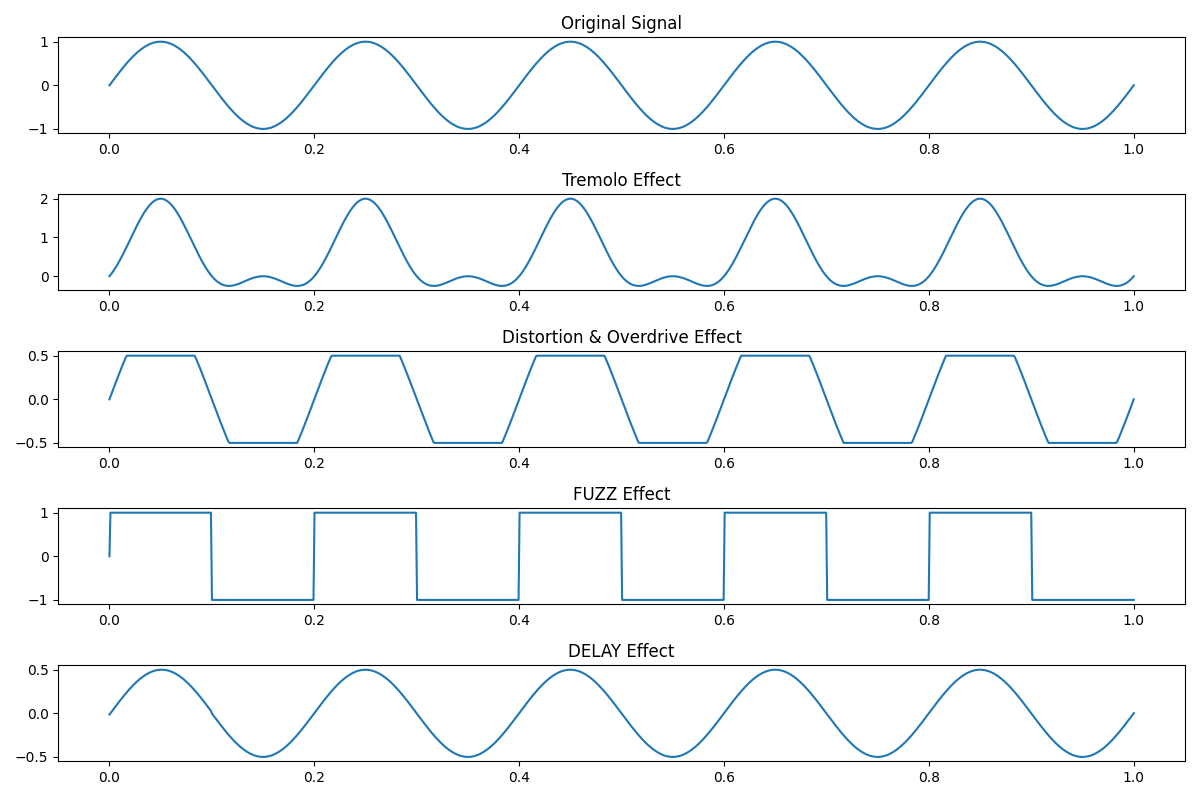
\includegraphics[width=\textwidth]{FPGA_waves.png}
    \caption{FPGA Waves: This figure shows the waveform outputs for different guitar effects as configured on the FPGA. Each waveform corresponds to a specific effect such as Tremolo, Distortion, FUZZ, Delay, etc., and illustrates how the signal is modified by each effect.}
    \label{fig:fpga_waves}
\end{figure}

\section{Implementation Details}
The effects were implemented using a combination of a soft-core processor and custom FPGA modules:
\begin{itemize}
    \item \textbf{Tremolo and Delay:} These effects were implemented using a soft-core processor. The processor handles the real-time processing required for these effects.
    \item \textbf{Distortion, Overdrive, and FUZZ:} These effects were implemented as custom FPGA modules. The FPGA handles the high-speed processing required for these effects.
\end{itemize}

\section{Effect Configuration}
\begin{itemize}
    \item All effects are configured with switches 0-3.
    \item To add an effect to the effect chain, flip switch 9.
    \item To clear the effect chain, flip the clear switch to the 1 position (see Figure \ref{fig:fpga_waves}).
    \item The effect properties are changed using KEY3 and KEY2 to lower or raise the value (see Figure \ref{fig:key3_and_2}).
    \item The 0’s and 1’s next to the effect name correspond to the positions of SW0-SW3 (see Figure \ref{fig:controls_keys_and_switches}).
    \begin{itemize}
        \item \textbf{0000 – Tremolo:} Amplitude modulation frequency changed with buttons 3 \& 2.
        \item \textbf{0001 – Distortion:} Cut off amplitude changed with buttons 3 \& 2.
        \item \textbf{0010 – Booster:} Volume boost configured with buttons 3 \& 2.
        \item \textbf{0011 – FUZZ:} Cut off amplitude changed with buttons 3 \& 2.
        \item \textbf{0100 – Overdrive:} Cut off amplitude changed with buttons 3 \& 2.
        \item \textbf{0101 – Delay:} Length of delay ranges between 1 second and 1/10 second.
        \item \textbf{0110 - Reverse Queue:} Length of queue ranges between 1 second and 1/10 second.
    \end{itemize}
\end{itemize}

\begin{figure}[h]
    \centering
    \includegraphics[width=0.5\linewidth]{key3_and_2.png}
    \caption{Effect properties are changed using KEY3 and KEY2.}
    \label{fig:key3_and_2}
\end{figure}

\begin{figure}[h]
    \centering
    \includegraphics[width=0.5\linewidth]{controlls_keys_and_switches.png}
    \caption{Controls for keys and switches.}
    \label{fig:controls_keys_and_switches}
\end{figure}

\begin{figure}[h]
    \centering
    \includegraphics[width=0.5\linewidth]{Power_button.png}
    \caption{Power button configuration.}
    \label{fig:power_button}
\end{figure}

\begin{figure}[h]
    \centering
    \includegraphics[width=0.5\linewidth]{Audio_in_out.png}
    \caption{Audio input and output configuration.}
    \label{fig:audio_in_out}
\end{figure}

\begin{figure}[h]
    \centering
    \includegraphics[width=0.5\linewidth]{example_sequence.png}
    \caption{Example sequence of effect configuration.}
    \label{fig:example_sequence}
\end{figure}

\bibliographystyle{plain}
\bibliography{references}

\end{document}